%%%%%%%%%%%%%%%%%%%%%%% file template.tex %%%%%%%%%%%%%%%%%%%%%%%%%
%
% This is a template file for the global option of the SVJour class
%
% Copy it to a new file with a new name and use it as the basis
% for your article
%
%%%%%%%%%%%%%%%%%%%%%%%% Springer-Verlag %%%%%%%%%%%%%%%%%%%%%%%%%%
%
% First comes an example EPS file -- just ignore it and
% proceed on the \documentclass line
\begin{filecontents*}{example.eps}
%!PS-Adobe-3.0 EPSF-3.0
%%BoundingBox: 19 19 221 221
%%CreationDate: Mon Sep 29 1997
%%Creator: programmed by hand (JK)
%%EndComments
gsave
newpath
  20 20 moveto
  20 220 lineto
  220 220 lineto
  220 20 lineto
closepath
2 setlinewidth
gsave
  .4 setgray fill
grestore
stroke
grestore
\end{filecontents*}
%
% Choose either the first of the next two \documentclass lines for one
% column journals or the second for two column journals.
%\documentclass[global,referee]{svjour}
\documentclass[global,twocolumn]{svjour}
%\documentclass[global,twocolumn]{svjour}
% Remove option referee for final version

\usepackage{graphicx}
\usepackage{epsfig}

\usepackage{graphics}
\usepackage{amssymb}
\usepackage{color}
\usepackage{listings}
\usepackage{pslatex}
\usepackage{subtable}
\usepackage{multirow}
\usepackage{url}
\usepackage[normalem]{ulem}
\usepackage{./styles/lstlang0}
\usepackage{./styles/lstAlloy}


% Insert the name of "your" journal with the command below:
\journalname{Software and System Modeling}

\begin{document}
\makeatletter


\newcommand{\nm@basicalert}[2]{\fbox{\bfseries\sffamily\scriptsize#1}{\sf\small$\blacktriangleright$\textit{#2}$\blacktriangleleft$}   }

\newcommand{\Naouel}[1]{\nm@basicalert{Naouel}{#1}}
\newcommand{\Cyril}[1]{\nm@basicalert{Cyril}{#1}}
\newcommand{\Sagar}[1]{\nm@basicalert{Sagar}{#1}}
\newcommand{\Olivier}[1]{\nm@basicalert{Olivier}{#1}}

\newcommand{\ie}{\textit{i.e.},}
\newcommand{\eg}{\textit{e.g.},}
\newcommand{\OCL}{\textsf{OCL}}

\newcommand{\nm@product}[1]{\textsc{#1}}
\newcommand{\nm@code}[1]{{\texttt{#1}}}
\newcommand{\nm@pattern}[1]{{\textsf{#1}}}
	\newcommand{\textGG}{\textsf{Graph Grammar}}
	\newcommand{\GG}{\textsf{GG}}
	\newcommand{\DCSP}{\textsf{DCSP}}
	\newcommand{\Graph}{\textsf{Graph}}
	\newcommand{\HFSM}{\textsf{HFSM}}
	\newcommand{\textHFSM}{\textsf{Hierarchical Finite State Machine}}
	\newcommand{\BNF}{\textsf{BNF}}
	\newcommand{\textBNF}{\textsf{Backus-Naur Form}}
	\newcommand{\textUMLCD}{\textsf{Unified Modelling Language Class Diagram}}
	\newcommand{\textUML}{\textsf{Unified Modelling Language}}
	\newcommand{\Prolog}{\textsf{Prolog}}
	\newcommand{\UMLCD}{\textsf{UMLCD}}
	\newcommand{\UML}{\textsf{UML}}
	\newcommand{\textOCL}{\textsf{Object Constraint Language}}
	\newcommand{\EMOF}{\textsf{EMOF}}
	\newcommand{\MOF}{\textsf{MOF}}
	\newcommand{\textMOF}{\textsf{Meta-object Facility}}
	\newcommand{\textEMOF}{\textsf{Essential Meta-object Facility}}
	\newcommand{\MDE}{MDE}
	\newcommand{\OMG}{\textsf{OMG}}
	\newcommand{\textOMG}{\textsf{Object Management Group}}
	\newcommand{\textMDE}{\emph{Model Driven Engineering}}
	\newcommand{\Float}{\textsf{Float}}
	\newcommand{\Boolean}{\textsf{Boolean}}
	\newcommand{\Integer}{\textsf{Integer}}
	\newcommand{\String}{\textsf{String}}
	\newcommand{\Himesis}{\textsf{Himesis}}
	\newcommand{\mmhfsm}{\textsf{MM}$_{\texttt{HFSM}}$}
	\newcommand{\mhfsm}{\textsf{m}$_{\texttt{HFSM}}$}
	\newcommand{\mhfsmc}{\textsf{m}$_{\texttt{HFSMConcrete}}$}
	\newcommand{\mmemof}{\textsf{MM}$_{\texttt{EMOF}}$}
	\newcommand{\mmtrace}{\textsf{MM}$_{\texttt{Trace}}$}
	\newcommand{\mexecution}{\textsf{m}$_{\texttt{Execution}}$}
	\newcommand{\mmgg}{\textsf{MM}$_{\texttt{GG}}$}
	\newcommand{\mConcrete}{K(\textsf{m}$_{\texttt{HFSMConcrete}}$)}
	\newcommand{\mtrace}{\textsf{m}$_{\texttt{Trace}}$}
	\newcommand{\mmggrule}{\textsf{MM\_2\_GG\_RuleGenerator}}
	\newcommand{\ASG}{\textsf{ASG}}
	\newcommand{\State}{\textsf{State}}
	\newcommand{\textSC}{\textsf{Statechart}}
	\newcommand{\Matches}{\textsf{Matches}}
	\newcommand{\textERD}{\textsf{Entity-relationship Diagram}}
	\newcommand{\textCD}{\textsf{Class Diagram}}
	\newcommand{\CD}{\textsf{CD}}
	\newcommand{\eclipse}{\textsf{ECLiPSe}}
	\newcommand{\prolog}{\textsf{{\Prolog}}}
	\newcommand{\classTransition}{\textbf{Transition}}
	\newcommand{\classState}{\textbf{State}}
	\newcommand{\classAbstractState}{\textbf{AbstractState}}
	\newcommand{\classHFSM}{\textbf{HFSM}}
	\newcommand{\classComposite}{\textbf{Composite}}
	\newcommand{\textCLP}{\textsf{Constraint Logic Programming}}
	\newcommand{\CLP}{\textsf{CLP}}
	\newcommand{\XML}{\textsf{XML}}
	\newcommand{\textXML}{\textsf{EXtended Markup Language}}
	\newcommand{\XMI}{\textsf{XMI}}
	\newcommand{\textXMI}{\textsf{XML Metadata Interchange}}
	\newcommand{\textRDBMS}{\textsf{Relational Database Management Systems}}
	\newcommand{\RDBMS}{\textsf{RDBMS}}
	\newcommand{\transfo}{\textsf{class2rdbms}}
	\newcommand{\ecore}{\textsf{Ecore}}
	\newcommand{\Class}{\textsf{Class}}
	\newcommand{\Attribute}{\textsf{Attribute}}
	\newcommand{\PrimitiveDataType}{\textsf{PrimitiveDataType}}
	\newcommand{\Association}{\textsf{Association}}
	\newcommand{\Property}{\textsf{Property}}
	\newcommand{\Model}{\textsf{Model}}
	\newcommand{\ClassModel}{\textsf{ClassModel}}
	\newcommand{\Classifier}{\textsf{Classifier}}


	\newcommand{\AllRanges}{\textsf{AllRanges}}
	\newcommand{\AllPartitions}{\textsf{AllPartitions}}
	\newcommand{\Unguided}{\textsf{Unguided}}

\newcommand{\red}[1]{{\color{red}#1}}
\newcommand{\blue}[1]{{\color{blue}#1}}

\def\Kermeta{Kermeta}
\def\Eclipse{\nm@product{Eclipse}}
\def\Ecore{\nm@product{Ecore}}
\def\Java{Java}
\def\UML{\nm@product{Uml}}
\def\Alloy{\nm@product{Alloy}}
\def\Cartier{\nm@product{Cartier}}
\def\Pramana{\nm@product{Pramana}}



\lstdefinestyle{numbers} {numbers=left, stepnumber=1, numberstyle=\tiny, numbersep=8pt}

\lstdefinestyle{nonumbers} {numbers=none}

%\title{Automatic Model Generation to Test Transformations}
\title{Automatic Test Model Generation to Transformation Pre-condition Refinement}
%\subtitle{A Symbiotic Methodology To Validate Model Transformations}


\author{Sagar Sen \and Jean-Marie Mottu \and Juan Cadavid \and Benoit Baudry 
% \thanks{\emph{Present address:} Insert the address here if needed}%
}

%
%\offprints{}          % Insert a name or remove this line
%

\author{Sagar Sen, Jean-Marie Mottu, Juan Cadavid, Benoit Baudry}

\institute{
	ATLANMOD, Ecole des Mines, 44000 Nantes, France\\
	\email{sagar.sen@mines-nantes.fr} \\
	Universit\'e de Nantes (IUT de Nantes / LINA - UMR CNRS 6241), \\
	3 rue du Mar\'{e}chal Joffre - 44000 Nantes\\
	\email{jean-marie.mottu@univ-nantes.fr} \\
    INRIA Rennes - Bretagne Atlantique / IRISA, Universit\'{e} Rennes 1,\\
    Triskell Team, Campus de Beaulieu, 35042 Rennes Cedex, France\\
    \email{\{jcadavid, bbaudry\}@irisa.fr} }
	



\date{Received: date / Revised version: date}
% The correct dates will be entered by the editor
%
\maketitle
%

\begin{abstract}

	
	Testing a \emph{model transformation} requires input test models which effectively cover the input domain of the transformation. In order to reduce testing costs and increase error-revealing power of test models, it is necessary to automate the generation of these models using systematic criteria.This automation faces two key challenges: (1) accurate specification of  the  transformation's input domain (2) automatic generation of  test models in the input domain based on effective coverage criteria. This paper presents a global approach that addresses these challenges. Typically the input domain defines a possibly infinite set of models specified using various sources of knowledge: the input metamodel of the transformation, static semantic constraints on this metamodel and pre-conditions that further constrain the input domain for a particular transformation. We use our tool {\Pramana} to automatically generate a finite number of test models in the input domain using coverage criteria based on partitioning properties of the input metamodel. Testing the transformation with these models often reveals that some test models are not executable by the transformation although they satisfy the constraints of the input domain specification. This gives way to incremental refinement of the input domain specification using newly constructed pre-conditions until all generated test models are executable by the transformation. In our experiments, we validate the proposed approach with mutation analysis to empirically evaluate error-revealing power of the test models we generate using {\Pramana}. The empirical evaluation uses the representative transformation of simplified UML class diagram models to RDBMS models. The evaluation is based on  3200 automatically generated test models. We demonstrate that partitioning strategies gives mutation scores of up to 93\% vs. 72\% in the case of unguided generation.

\end{abstract}

\section{Introduction}
\label{section:Introduction}

Model transformations are core {\textMDE} ({\MDE}) components that automate important steps in software development such as refinement of an input model, re-factoring to improve maintainability or readability of the input model, aspect weaving into models, exogenous/endogenous transformations of models, and the classical generation of code from models. Although there is wide spread development of model transformations in academia and industry. However, there is mild progress in techniques to test transformations \cite{Baudry09a}. In this paper, we address the problem of testing model transformations using automatically generated  test models. Our approach is applicable to a diverse set of transformation languages such as those based on graph rewriting \cite{bardohl99}, imperative execution (Kermeta \cite{muller2005}), and rule-based transformation (ATL \cite{jouault2006}).

   
 Testing a model transformation requires a \emph{set of test models} in the input domain of a model transformation.   The automatic synthesis/generation of such test models that can reveal bugs in a transformation is the subject of this paper. 
 
 The automatic generation of test models selects test models from the set of all input models. This set of input models is precisely specified by the input domain of a model transformation. Typically, this input domain specification relies on knowledge from various sources: (1) the input metamodel of the transformation (2) invariants/constraints on the static semantics of the input metamodel (3) pre-condition contracts for a particular transformation.  We call the cumulative set of these sources of knowledge the \emph{input domain model}.  The input domain model  specifies potentially an infinite set of  input models. Therefore, we need to go a step further and define effective strategies, such as coverage criteria  \cite{franck2007}, that can help automatically select a finite number of  test models in the infinite set.  

In this paper, we build on previous work \cite{sen2008} to automatically generate test models using the tool {\Pramana} (previously known as {\Cartier}) within the input domain of a transformation. Executing the model transformation with these test models often results in some test models being rejected by the transformation. Although these test models conform to the initial specification of the input domain model, they are rejected by the transformation. This may happen when the transformation runs into an infinite cyclic loop while navigating an input model. At this point there are two possibilities: (a) Modifying a model transformation's specification and consequently its implementation to handle such an input model (b) Creating a pre-condition that avoids input models with a certain pattern such as a loop. This is a dilemma about whether to correct a model transformation to make it robust or improve the pre-condition to handle unforeseen inputs. The choice of one approach or the other depends on how we would like to interprets the specification. In this paper, we consider taking step (b) to identify the \emph{true input domain} of a model transformation conforming to a specification.  Our \emph{first contribution} in the paper is as follows:

\textbf{Incremental Pre-condition Improvement}: We automatically generate test models using {\Pramana} to first identify test models outside the unknown \emph{true} input domain of a model transformation. We  systematically compose new pre-conditions using information  extracted from a  malicious pattern in the generated test models. We improve the current set of pre-conditions of the model transformation. We use the new specification of the input domain model to generate test models and improve the set of pre-conditions. We continue the process until no new pre-condition is required and all generated test models can be executed by the transformation. The output of the process is the precise model of the true input domain of a model transformation. Pre-condition improvement is an approach adapted to black-box transformations where we have no access to the implementation. It also reveals the unforeseen requirements in case we want to evolve a model transformation. Therefore, a pre-condition may be converted to a new model transformation feature. We see pre-condition improvement as either a means to protect the model transformation or to extract requirements in the form of constraints/rules for the evolution of the transformation.

Once, we have a precise input domain model the consequent next step is to generate new test models. This time to detect bugs in a transformation. This brings us to the \emph{second contribution} of the paper:

\textbf{Automatic Generation and Evaluation of Test Models}: We first use {\Pramana} to generate sets of  test models for different strategies in the precise input domain of a model transformation. In this paper, we generate test models that satisfy coverage criteria \cite{franck2007}.  Second, we use \emph{mutation analysis} \cite{demillo1978} \cite{mottu2006} for model transformations as technique to evaluate if these test sets can indeed reveal bugs. Mutation analysis consists of artificially injecting \emph{model transformation specific} bugs into a model transformation giving a set of mutant model transformations with exactly one bug in each mutant. We execute each of these mutants with a set  of generated test models for a given strategy. A difference in output between the original transformation and a mutant transformation reveals that an error was detected for the same input test model. Consequently, the number of such errors detected by a set of test model refers to the \emph{mutation score} of the test set. This number of errors detected corresponds to the \emph{mutation score} of a test set which is the metric we use to compare test generation strategies. Mutation analysis is done mainly to evaluate the effectiveness of our coverage criteria to generate test models that detect bugs. However, mutation analysis is not used in practice for testing. We use mutation analysis to gain confidence that test models generated with {\Pramana} can detect bugs for the representative transformation. Based on our mutation analysis results we encourage  generation of test models using our coverage criteria in new scenarios involving arbitrary input domains and transformations.

We demonstrate incremental pre-condition improvement and empirically evaluate automatic test model generation for  the  representative model transformation of {\textUMLCD} ({\UMLCD}) to {\textRDBMS}  ({\RDBMS}) models called {\transfo}.  We discover nine new pre-conditions for the {\transfo}. Using mutation analysis we demonstrate that  our input domain coverage strategies, previously presented in \cite{franck2007}, can  select test models with considerably higher bug detection abilities (93\%) compared to unguided selection (72\%) in the input domain.. These results are based on 3200 generated test models and several hours of computation on a 10 machine grid of high-end servers.  The large difference in mutation scores between coverage strategies and unguided selection can be attributed to  the fact that coverage strategies enforce several aspects on test models that unguided selection fails to do. For instance, coverage strategies enforce injection of \emph{inheritance} in the {\UMLCD} test models. Unguided strategies do not enforce such a requirement. Several mutants are killed due to test models containing inheritance. 
	 

The paper is organized as follows. In Section \ref{sec:ProblemDescription} we present the transformation testing problem and the running case study. In Section \ref{sec:Foundation}, we present foundational ideas used in {\Pramana}. In  Section \ref{sec:Methodology}, we describe the {\Pramana} methodology for incremental pre-condition improvement and the empirical approach for automatic test model generation. In Section \ref{sec:Experiments}, we present the experimental setup for test model generation using different strategies and discuss the results of mutation analysis. In Section \ref{sec:RelatedWork} we present related work. We conclude in Section \ref{sec:Conclusion}.

\section{Problem Description}
\label{sec:ProblemDescription}

We present the problem of  testing \emph{model transformations}. A model transformation $MT(I,O)$ is a program applied on a set of input models $I$ to produce a set of output models $O$ as illustrated in Figure \ref{fig:exampleAndMT}. The set of all input models is specified by a metamodel $MM_{I}$ (For example, simplified {\UMLCD} in Figure \ref{fig:umlcd}). The set of all output models is specified by metamodel $MM_{O}$. The pre-condition of the model transformation $pre(MT)$ further constrains the input domain. A post-condition $post(MT)$ constrains the model transformation to producing a subset of all possible output models. The model transformation is developed based on a set of textual specification of requirements $MT_{Requirements}$.

\begin{figure} [!t]
\begin{center}

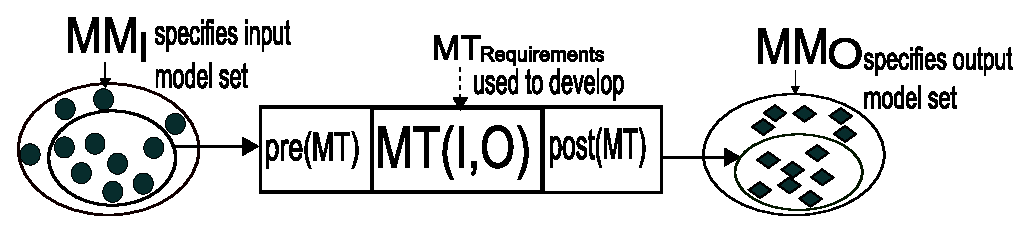
\includegraphics[width=3.5 in]{./figures/modelTransformation.eps}
\end{center}

\caption{A Model Transformation}
\label{fig:exampleAndMT}

\end{figure}

Automatic model generation for testing involves finding valid input models we call \emph{test models} from the set of all input models $I$. Test models must  satisfy constraints that increase the trust in the quality of these models as test data and thus should increase their capabilities to detect bugs in the model transformation $MT(I,O)$. Bugs may also exist in the input metamodel and its invariants $MM_{I}$ or the transformation pre-condition $pre(MT)$. However, in this paper we only focus on generating input models that can detect bugs in a transformation. In the process, we also generate input models that cannot be processed by a transformation (as they were unforeseen in $MT_{Requirements}$) which are then used to specify new pre-conditions.

\subsection{Transformation Case Study}

Our case study is the transformation from simplified {\UML} Class Diagram models to {\RDBMS} models called {\transfo}.  In this section we briefly describe {\transfo} and discuss why it is a representative transformation to validate test model generation strategies.

In testing we need input models that conform to the input metamodel $MM_{I}$ and transformation pre-condition $pre(MT)$. Therefore, we only discuss the $MM_{I}$ and $pre(MT)$ for {\transfo} and avoid discussion of the model transformation output domain. In Figure \ref{fig:umlcd}, we present the simplified {\UMLCD} input metamodel for {\transfo}. The concepts and relationships in the input metamodel are stored as an {\ecore} model \cite{emf2004} (Figure \ref{fig:umlcd} (a)). The invariants on the simplified {\UMLCD} {\ecore} model, expressed in {\textOCL} ({\OCL}) \cite{OCL}, are shown in Figure \ref{fig:umlcd} (b). The {\ecore} model and the invariants together represent the input domain for {\transfo}. The {\OCL} and {\ecore} are industry standards used to develop metamodels and specify different invariants on them. {\OCL} is not a domain-specific language to specify invariants. However, it is designed to formally encode natural language requirements specifications independent of its domain. 
%In \cite{oclShort} the authors present some limitations of {\OCL}.

The input metamodel $MM_{I}$ gives an initial specification of the input domain. However, the model transformation itself has a pre-condition $pre(MT)$ that test models need to satisfy to be correctly processed. Constraints in the pre-condition for {\transfo} include: (a) All {\Class} objects must have at least one primary {\Property} object (b) The type of an {\Property} object can be a {\Class} C, but finally the transitive closure of the type of {\Property} objects of {\Class} C must end with type {\PrimitiveDataType}. In our case we approximate this recursive closure constraint by stating that {\Property} object can be of type {\Class} up to a depth of 3 and the 4th time it should have a type {\PrimitiveDataType}. This is a finitization operation to avoid navigation in an infinite loop. (c) A {\Class} object cannot have an {\Association} and an {\Property} object of the same name (d) There are no cycles between non-persistent {\Class} objects.

We choose {\transfo} as our representative case study to validate input selection strategies. It serves as a sufficient case study for several reasons. The transformation is the benchmark proposed in the MTIP workshop at the MoDELS 2005 conference \cite{bezivin2005} to experiment and validate model transformation language features. The input domain metamodel of simplified {\UMLCD}  covers all major metamodelling concepts such as inheritance, composition, finite and infinite multiplicities. The constraints on the simplified {\UMLCD} metamodel contain both first-order and higher-order constraints. There also exists a constraint to test transitive closure properties on the input model such as there must be no cyclic inheritance. The {\transfo} exercises most major model transformation operators such as navigation, creation, and filtering (described in more detail in \cite{mottu2006}) enabling us to test essential model transformation features. Among the limitations the simplified  {\UMLCD} metamodel does not contain {\Integer} and {\Float} attributes. There are also no inter-metamodel references and arbitrary containments in the simple metamodel. 

\begin{figure*} [!t]
\begin{center}
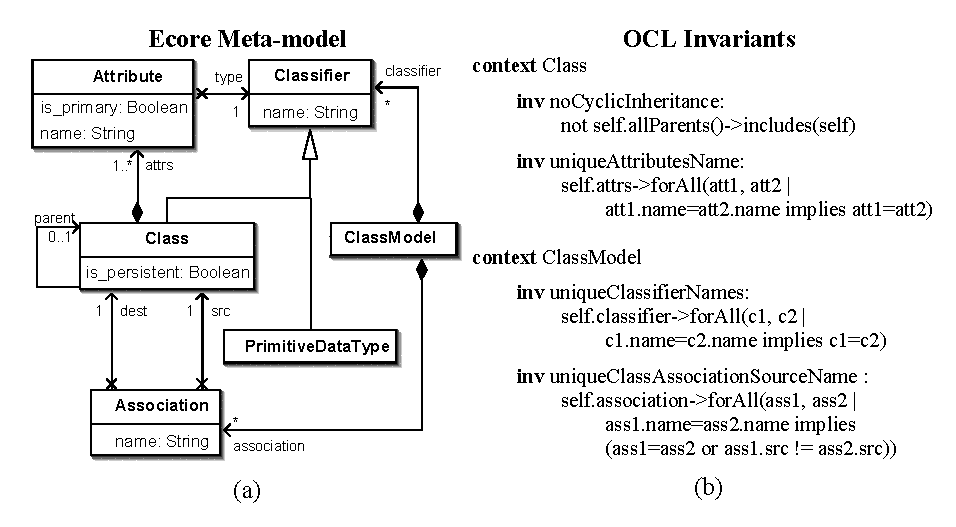
\includegraphics[scale=0.75]{./figures/classMMwithInv.eps}
\end{center}
\caption{(a) Class Diagram Subset of {\UML} {\ecore} Meta-model (b) {\OCL} constraints on the {\ecore} metamodel}
\label{fig:umlcd}

\end{figure*}

Model generation is relatively fast but performing mutation analysis is extremely time consuming. Therefore, we perform mutation analysis on {\transfo} to qualify transformation and metamodel independent strategies for model synthesis. If these strategies prove to be useful in the case of {\transfo} then we recommend the use of these strategies to guide model synthesis in the input domain of other model transformations as an initial test generation step. For instance, in our experiments, we see that generation of a 15 class simplified {\UMLCD} models takes about 20 seconds and mutation analysis of a set of 20 such models takes about 3 hours on a multi-core high-end server. Generating thousands of models for different transformations takes about 0.25\% of the time while performing mutation analysis takes most of the time. 
\section{Foundations}
\label{sec:Foundation}


This section presents foundational ideas used by the methodology for automatic test model generation and empirical evaluation presented in Section \ref{sec:Methodology}.  First, we present the modelling and model transformation language {\Kermeta} in Section \ref{sec:sec:Kermeta}. We use {\Kermeta} to implement all model transformations in the paper. We briefly describe {\Pramana} for automatic test model generation in Section \ref{sec:sec:transfo2Alloy}. Effective test model generation in this paper is guided by coverage criteria based testing strategies. These testing strategies are described in Section \ref{sec:sec:testStrategy}. Finally, the bug detecting effectiveness of  test models generated using different testing strategies is
done by mutation analysis. Mutation analysis for model transformations is described in Section \ref{sec:sec:ma}.

\subsection{Kermeta}
\label{sec:sec:Kermeta}

\Kermeta{} is a language for specifying metamodels, models, and model transformations that are compliant to the Meta Object Facility (MOF) standard \cite{MOF2}. The object-oriented meta-language MOF supports the definition of metamodels in terms of object-oriented structures (packages, classes, properties, and operations). It also provides model-specific constructions such as containments and associations between classes. \Kermeta{} extends the MOF with an \emph{imperative action language} for specifying constraints and operational semantics for metamodels \cite{Muller05a}. \Kermeta{} is built on top of EMF within the \Eclipse{} development environment. The action language of \Kermeta{} provides mechanisms for dynamic binding, reflection, and exception handling. It also includes classical control structures such as blocks, conditionals, and loops.


\subsection{{\Pramana}: A Tool for Automatic Model Generation}
\label{sec:sec:transfo2Alloy}

We use the tool {\Pramana} previously introduced (with the name {\Cartier}) in our paper \cite{sen2008} to automatically generate test models. {\Pramana} transforms the input domain specification of a model transformation to a common constraint language {\Alloy}. Solving the {\Alloy} model gives zero or more models in the input domain of a transformation. {\Pramana} first transforms a model transformation's  input metamodel expressed in the Eclipse Modelling Framework \cite{emf2004} format called Ecore using the transformation rules presented in \cite{sen2008} to {\Alloy}. Basically, classes in the input metamodel are transformed to {\Alloy} signatures and implicit constraints such as inheritance, opposite properties, and multiplicity constraints are transformed to {\Alloy} facts. 

Second, {\Pramana} also addresses the issue of transforming invariants and pre-conditions on metamodels expressed in the industry standard {\textOCL} ({\OCL}) to {\Alloy}. The automatic transformation of  {\OCL} to {\Alloy} presents a number of challenges that are discussed in \cite{AnastasakisBGR07}. We do not claim that all {\OCL} constraints can be manually/automatically transformed to {\Alloy} for our approach to be applicable in the most general case. The reason being that {\OCL} and {\Alloy} were designed with different goals. {\OCL} is used mainly to query a model and check if certain invariants are satisfied. {\Alloy} facts and predicates on the other hand enforce constraints on a model. This is in contrast with the side-effect free {\OCL}. The core of {\Alloy} is declarative and is based on first-order relational logic with quantifiers while {\OCL} includes higher-order logic and has imperative constructs to call operations and messages making some parts of {\OCL} more expressive. In our case study, we have been successful in transforming all meta-constraints on the {\UMLCD} metamodel to {\Alloy} from their original {\OCL} specifications. Nevertheless, we are aware of {\OCL}'s status as a current industrial standard and thus provide an automatic mapping to complement our approach.


Previous work exists in mapping {\OCL} to {\Alloy}. The tool UML2Alloy \cite{anastasakis2009} takes as input {\UML} class models with {\OCL} constraints. The authors present a set of mappings between {\OCL} collection operations and their {\Alloy} equivalents. Here we present our version of such transformation derived from \cite{anastasakis2009} and written in  {\Kermeta}.

The context of an {\OCL} constraint (which is what defines the value of the \emph{self} constraint) determines the place of the constraint within the generated {\Alloy} model. It is added as an appended fact. The mappings in Table \ref{table:ocl2alloy} (taken in part from \cite{anastasakis2009}) show the automatic transformation rules applied in {\Pramana}.

\begin{table} [!b]
%% increase table row spacing, adjust to taste
\renewcommand{\arraystretch}{1}
\renewcommand{\arrayrulewidth}{1 pt}
\caption{Mappings from {\OCL} to {\Alloy}}
\label{table:ocl2alloy}
%\centering   
\begin{tabular}{p {8cm}}
Let \emph{v} be a variable,
\emph{col} a collection,
\emph{expr} an expression,
\emph{be} an expression that returns a boolean value,
\emph{o} an expression that returns an object,
\emph{T} a type,              
\emph{propertyCallExpr} an expression invoking a property on an object
\end{tabular}
\begin{tabular}{p {4 cm} p {4 cm}}
\hline
\textbf{ {\OCL} Expression Type} & \textbf{{\Alloy} Abstract Syntax Type }\\
\hline
$context\ T\ inv\ expr$ & $sig\ T \{{\ldots}\}\{expr\}$ \\
$col \to forAll(v : T \mid be)$ & $all\ v : T \mid be$ \\
$col \to forAll(v : col \mid be)$ & $all\ v : col \mid be$ \\
$expr1 and expr2$ & $expr1\ \&\&\ expr2$ \\
$expr1 or expr2$ & $expr1 \mid\mid expr2$ \\
$not\ be$ & $!be$ \\
$col \to size()$ & $\#col$ \\
$col \to includes(o : T)$ & $o\ in\ col$ \\
$col \to excludes(o : T)$ & $o\ !in\ col$ \\
$col1 \to includesAll(col2)$ & $col2\ in\ col1$ \\
$col1 \to excludesAll(col2)$ & $col2\ !in\ col1$ \\
$col \to including(o : T)$ & $col\ +\ o$ \\
$col \to excluding(o : T)$ & $col\ -\ o$ \\
$col \to isEmpty()$ & $no\ col$ \\
$col \to notEmpty()$ & $some\ col$ \\
$expr.propertyCallExpr$ & $expr.propertyCallExpr$ \\
$if\ be\ then\ expr1\ else\ expr2$ & $be \Rightarrow expr1\ else\ expr2$ \\
$expr.oclIsUndefined$ & $\#expr = 0$ \\
$expr \to oclIsKindOf(o : T)$ & $expr\ in\ o$ \\
$col1 \to union(col2)$ & $col1 + col2$ \\
$col1 \to intersection(col2)$ & $col1\ \&\ col2$ \\
$col1 \to product(col2)$ & $col1 \to col2$ \\
$col \to sum()$ & $sum\ col$ \\
$col1 \to symmetricDifference(col2)$ & $(col1 + col2) - (col1 \& col2)$\\
$col \to select(be)$ & $v : col \mid be $\\
$col \to isUnique(propertyCallExpr)$ & $no\ disj\ v1,\ v2 : col \mid
v1.propertyCallExpr = v2.propertyCallExpr$ \\
\hline
\end{tabular}

\end{table}



However, some classes of {\OCL} invariants cannot be automatically transformed to {\Alloy} using the simple rules in Table \ref{table:ocl2alloy}. For example, consider the invariant for no cyclic inheritance in Figure \ref{fig:umlcd}(b) \cite{baar2003}. The constraint is specified as the fact in Listing \ref{listing:alloyfact}. This is an example in which the richness of the {\Alloy} language overcomes {\OCL} - it is not possible to specify this constraint in {\OCL} without using recursive queries since there is no transitive closure operator.


\lstinputlisting[language=Alloy, basicstyle=\tiny,
style=nonumbers, frame=single, framerule=0.2pt, captionpos=b,
caption={{\Alloy} Fact for No Cyclic Inheritance}, label={listing:alloyfact}]{./listings/exampleOCLAlloyFact.tex}


The generated {\Alloy} model for the {\UMLCD} metamodel using {\Pramana} is given in Appendix \ref{appendix:mainmodel}. This {\Alloy} model describes the  input domain of the transformation. 

\subsection{Test Selection Strategies}
\label{sec:sec:testStrategy}

Effective strategies to guide automatic model generation are required to select test models that detect bugs in a model transformation. We define a strategy as a process that generates \emph{{\Alloy} predicates} which are constraints added to the {\Alloy} model synthesized by {\Pramana} as described in Section \ref{sec:Methodology}. This combined {\Alloy} model is solved and the solutions are transformed to model instances of the input metamodel that satisfy the predicate. We present the following strategies to guide model generation:

\begin{itemize}
	\item \textbf{Random/Unguided Strategy:} The basic form of model generation is unguided where only the {\Alloy} model obtained from the metamodel and transformation is used to generate models. No extra knowledge is supplied to the solver in order to generate models. The strategy yields an empty {\Alloy} predicate as shown in Listing \ref{listing:emptypred}.
	
	\lstinputlisting[language=Alloy, basicstyle=\tiny,
style=nonumbers, frame=single, framerule=0.2pt, captionpos=b,
caption={Empty {\Alloy} Predicate }, label={listing:emptypred}]{./listings/emptyAlloyPredicate.tex}


	\item \textbf{Input-domain Partition based Strategies:}
		We guide generation of models using test criteria to combine \emph{partitions} on domains of all properties of a metamodel (cardinality of references or domain of primitive types for attributes).  A \emph{partition} of a set of elements is a collection of $n$ ranges $A_1$,..., $A_n$ such that $A_1$, ..., $A_n$  do not overlap and the union of all subsets forms the initial set. These subsets are called \emph{ranges}. We use partitions of the input domain since the number of models in the domain are infinitely many. Using partitions of the properties of a metamodel we define two coverage criteria that are based on different strategies for combining partitions of properties. Each criterion defines a set of \emph{model fragments} for an input metamodel. These fragments are transformed to predicates on metamodel properties by {\Pramana}. For a set of test models to cover the input domain  at least one model in the set must cover each of these model fragments. We generate model fragment predicates using the following coverage criteria to combine partitions (cartesian product of partitions):
		\begin{itemize}
			\item \textbf{AllRanges Criteria:} {\AllRanges} specifies that each range in the partition of each property must be covered by at least one test model.
			\item \textbf{AllPartitions Criteria:} {\AllPartitions} specifies that the whole partition of each property must be covered by at least one test model.
		\end{itemize}

\end{itemize}

The notion of coverage criteria to generate model fragments was initially proposed in our paper \cite{franck2007}. The accompanying tool called Meta-model Coverage Checker (MMCC) \cite{franck2007} generates model fragments using different test criteria taking any metamodel as input. Then, the tool automatically computes the coverage of a set of test models according to the generated model fragments. If some fragments are not covered, then the set of test models should be improved in order to reach a better coverage. 

In this paper, we use the model fragments generated by MMCC for the {\UMLCD}  {\ecore} model (Figure \ref{fig:umlcd}). We use the criteria {\AllRanges} and {\AllPartitions}.   For example, in Table \ref{table:modelFrags}, \emph{mfAllRanges1} and \emph{mfAllRanges2} are model fragments generated by {\Pramana} using MMCC \cite{franck2007} for the \emph{name} property of a classifier object. The \emph{mfAllRanges1} states that there must be at least one classifier object with an empty name while \emph{mfAllRanges2} states that there must be at least one classifier object with a non-empty name. These values for name are the ranges for the property. The model fragments chosen using {\AllRanges} \emph{mfAllRanges1} and \emph{mfAllRanges2} define two partitions \emph{partition1} and \emph{partition2}. The model fragment  \emph{mfAllPartitions1} chosen using {\AllPartitions} defines both \emph{partition1} and \emph{partition2}.

\begin{table} [!b]
%% increase table row spacing, adjust to taste
\renewcommand{\arraystretch}{1}
\renewcommand{\arrayrulewidth}{1 pt}
\caption{Consistent Model Fragments Generated using {\AllRanges} and {\AllPartitions} Strategies}
\label{table:modelFrags}
%\centering
\begin{tabular}{p {2.5 cm} p {5.5 cm}}
\hline
\textbf{Model-Fragment} & \textbf{ Description} \\ \hline 
 mfAllRanges1 &  A {\Classifier}  $c \mid c.name=$``''\\%\begin{verbatim} some c:Classifier|c.name>=0 \end{verbatim}\\    
 mfAllRanges2 &  A {\Classifier}  $c \mid c.name!=$``''\\%\begin{verbatim} some c:Classifier|c.name>=0 \end{verbatim}\\   
 mfAllRanges3 & A {\Class}  $c \mid c.is\_persistent=True$ \\%\begin{verbatim}some c:Class |c.is_persistent=True\end{verbatim} \\
 mfAllRanges4 & A {\Class}  $c \mid c.is\_persistent=False$ \\%\begin{verbatim}some c:Class |c.is_persistent=False\end{verbatim} \\
 mfAllRanges5 & A {\Class}  $c \mid \#c.parent = 0$\\ %\begin{verbatim}some c:Class|#c.parent=0 \end{verbatim} \\
 mfAllRanges6 & A {\Class}  $c \mid \#c.parent = 1$\\ %\begin{verbatim}some c:Class|#c.parent=0 \end{verbatim} \\
 mfAllRanges7 & A {\Class}  $c \mid \#c.attrs=1$\\ %\begin{verbatim}some c:Class|#c.attrs=1\end{verbatim} \\
 mfAllRanges8 & A {\Class}  $c \mid \#c.attrs > 1$\\ %\begin{verbatim}some c:Class|#c.attrs>1\end{verbatim} \\
 mfAllRanges9 & An {\Attribute}  $a \mid a.is\_primary=True$\\ %\begin{verbatim}some a:Attribute|a.is_primary=True \end{verbatim}\\
 mfAllRanges10 & An {\Attribute}  $a \mid a.name=$``''\\% \begin{verbatim}some a:Attribute|a.name=0 \end{verbatim}\\
 mfAllRanges11 & An {\Attribute}  $a \mid a.name!=$``''\\%\begin{verbatim}some a:Attribute|a.name!=0 \end{verbatim}\\    
 mfAllRanges12 & An {\Attribute}  $a \mid \#a.type=1$\\ %\begin{verbatim}some a:Attribute|#a.type=1 \end{verbatim}\\
 mfAllRanges13 & An {\Association}  $as \mid as.name=$``''\\%\begin{verbatim}some a:Association|a.name=0  \end{verbatim}\\
 mfAllRanges14 & An {\Association}  $as \mid \#as.src=1$\\ %\begin{verbatim}some a:Association|#a.dest=1 \end{verbatim}  \\
 mfAllRanges15 & An {\Association}  $as \mid \#as.dest=1$\\ %\begin{verbatim}some a:Association|#a.dest=1 \end{verbatim} \\
 mfAllPartitions1 & {\Classifier}s  $c1,c2 \mid c1.name=$``'' and $c2.name!=$``'' \\ %\begin{verbatim}some c:Classifier|c.name=0 and some c:Classifier|c.name>=0\end{verbatim}\\
 mfAllPartitions2 & {\Class}es  $c1,c2 \mid c1.is\_persistent=True$ and $c2.is\_persistent=False $  \\ %\begin{verbatim}some c:Class |c.is_persistent=True and some c:Class |c.is_persistent=False\end{verbatim} \\
 mfAllPartitions3 & {\Class}es  $c1,c2 \mid \#c1.parent=0$ and $\#c2.parent=1$ \\ %\begin{verbatim}some c:Class|#c.parent=0 and some c:Class|#c.parent=1\end{verbatim} \\
 mfAllPartitions4 & {\Property}s $a1,a2 \mid a1.is\_primary=True$ and $a2.is\_primary=False$ \\ %\begin{verbatim}some a:Attribute|a.is_primary=True and some a:Attribute|a.is_primary=False and some a:Attribute|a.name=0 \end{verbatim}\\
 mfAllPartitions5 & {\Association}s $as1,as2 \mid as1.name=$``'' and $as2.name!=$``'' \\ %\begin{verbatim}some a:Association|a.name=0  and some a:Association|a.name!=0\end{verbatim} \\
\hline 
\end{tabular} 

\end{table}

These model fragments are transformed to {\Alloy} predicates by {\Pramana}. For instance, model fragment \emph{mfAllRanges7} is transformed to the predicate in Listing \ref{listing:mfpred}.

\lstinputlisting[language=Alloy, basicstyle=\tiny,
style=nonumbers, frame=single, framerule=0.2pt, captionpos=b,
caption={{\Alloy} Predicate for \emph{mfAllRanges7} }, label={listing:mfpred}]{./listings/exampleAlloyPredicate.tex}
	
	As mentioned in our previous paper \cite{franck2007} if a test set contains models where all model fragments are contained in at least one model then we say that the input domain is completely covered. However, these model fragments are generated considering only the concepts and relationships in the {\ecore} model and they do not take into account the constraints on the {\ecore} model. Therefore, not all model fragments are consistent with the input metamodel because the generated models that contain these model fragments do not satisfy the constraints on the metamodel. {\Pramana} invokes the {\Alloy} Analyzer \cite{alloy} to automatically check if a model containing a model fragment and satisfying the input domain can be synthesized for a general scope of number of objects. This allows us to \emph{detect inconsistent model fragments}. For example, the following predicate, \emph{mfAllRanges7a}, is the {\Alloy} representation of a model fragment specifying that some {\Class} object does not have any {\Property} object. {\Pramana} calls the {\Alloy} API to execute the run statement for the predicate \emph{mfAllRanges7a} along with the base {\Alloy} model to create a model that contains up to 30 objects per class/concept/signature (see Listing \ref{listing:mfpredrun}).
	
	
\lstinputlisting[language=Alloy, basicstyle=\tiny,
style=nonumbers, frame=single, framerule=0.2pt, captionpos=b,
caption={{\Alloy} Predicate and Run Command }, label={listing:mfpredrun}]{./listings/exampleAlloyPredicateRun.tex}
	

The {\Alloy} analyzer yields a \emph{no solution} to the run statement indicating that the model fragment is not consistent with the input domain specification. This is because no model can be created with this model fragment that also satisfies an input domain constraint that states that every {\Class} must have at least one {\Property} object as shown in Listing \ref{listing:alloysig}.

\lstinputlisting[language=Alloy, basicstyle=\tiny,
style=nonumbers, frame=single, framerule=0.2pt, captionpos=b,
caption={Example {\Alloy} Signature}, label={listing:alloysig}]{./listings/exampleAlloySig.tex}
	

In Listing \ref{listing:alloysig},  \emph{some} indicates 1..*.  However, if a model solution can be found using {\Alloy} we call it a \emph{consistent model fragment}. MMCC generates a total of 15 consistent model fragments using {\AllRanges} and 5 model fragments using the {\AllPartitions} strategy, as shown in Table \ref{table:modelFrags}.


\subsection{Qualifying Models: Mutation Analysis for Model Transformation Testing}
\label{sec:sec:ma}

We generate sets of test models using different strategies and qualify these sets via mutation analysis \cite{demillo1978}. Mutation analysis involves creating a set of faulty versions or \emph{mutants} of a program. A test set must distinguish the program output from all the output of its mutants. In practice, faults are modelled as a set of mutation operators where each operator represents a class of faults. A mutation operator is applied to the program under test to create each mutant. A mutant is killed when at least one test model detects the pre-injected fault. It is detected when program output and mutant output are different. A test set is relatively adequate if it kills all mutants of the original program.  A mutation score is associated to the test set to measure its effectiveness in terms of percentage of the killed/revealed mutants.

We use the mutation analysis operators for model transformations presented in our previous work \cite{mottu2006}. These mutation operators are based on three abstract operations linked to the basic treatments in a model transformation: the navigation of the models through the relations between the classes, the filtering of collections of objects, the creation and the modification of the elements of the output model. Using this basis we define several mutation operators that inject faults in model transformations:

\textbf{Relation to the same class change (RSCC): }The navigation of one association toward a class is replaced with the navigation of another association to the same class.

\textbf{Relation to another class change (ROCC): }The navigation of an association toward a class is replaced with the navigation of another association to another class.

\textbf{Relation sequence modification with deletion (RSMD): }This operator removes the last step off from a navigation which successively navigates several relations.

\textbf{Relation sequence modification with addition (RSMA): }This operator does the opposite of RSMD, adding the navigation of a relation to an existing navigation.

\textbf{Collection filtering change with perturbation (CFCP): }The filtering criterion, which could be on a property or the type of the classes filtered, is disturbed.

\textbf{Collection filtering change with deletion (CFCD): }This operator deletes a filter on a collection; the mutant operation returns the collection it was supposed to filter.

\textbf{Collection filtering change with addition (CFCA): }This operator does the opposite of CFCD. It uses a collection and processes an additional filtering on it.

\textbf{Class compatible creation replacement (CCCR): }The creation of an object is replaced by the creation of an instance of another class of the same inheritance tree.

\textbf{Classes association creation deletion (CACD): }This operator deletes the creation of an association between two instances.

\textbf{Classes association creation addition (CACA): }This operator adds a useless creation of a relation between two instances.

Using these operators, we produced two hundred mutants from the {\transfo} model transformation with the repartition indicated in Table \ref{table:mutation}.
%\begin{table*} [!t]
\begin{table*} 
\renewcommand{\arraystretch}{1}
\renewcommand{\arrayrulewidth}{1 pt}
\caption{Repartition of the {\transfo} mutants depending on the mutation
operator applied}
\label{table:mutation}
\centering
\begin{tabular}{l l  l l l l l l l l l}
\hline
\textbf{Mutation Operator} & CFCA & CFCD& CFCP
&CACD&CACA&RSMA&RSMD&ROCC&RSCC&Total \\ \hline 
\textbf{Number of Mutants}& 19&18&38&11&9&72&12&12&9&200\\ \hline
\end{tabular} 
\end{table*}

In general, not all mutants injected become faults as some of them are equivalent and can never be detected. The controlled experiments presented in this paper uses mutants presented in our previous work \cite{mottu2006}. We have clearly identified faults and equivalent mutants to study the effect of our generated test models.







\section{Methodology}
\label{sec:Methodology}


\begin{figure*} [!t]
\begin{center}
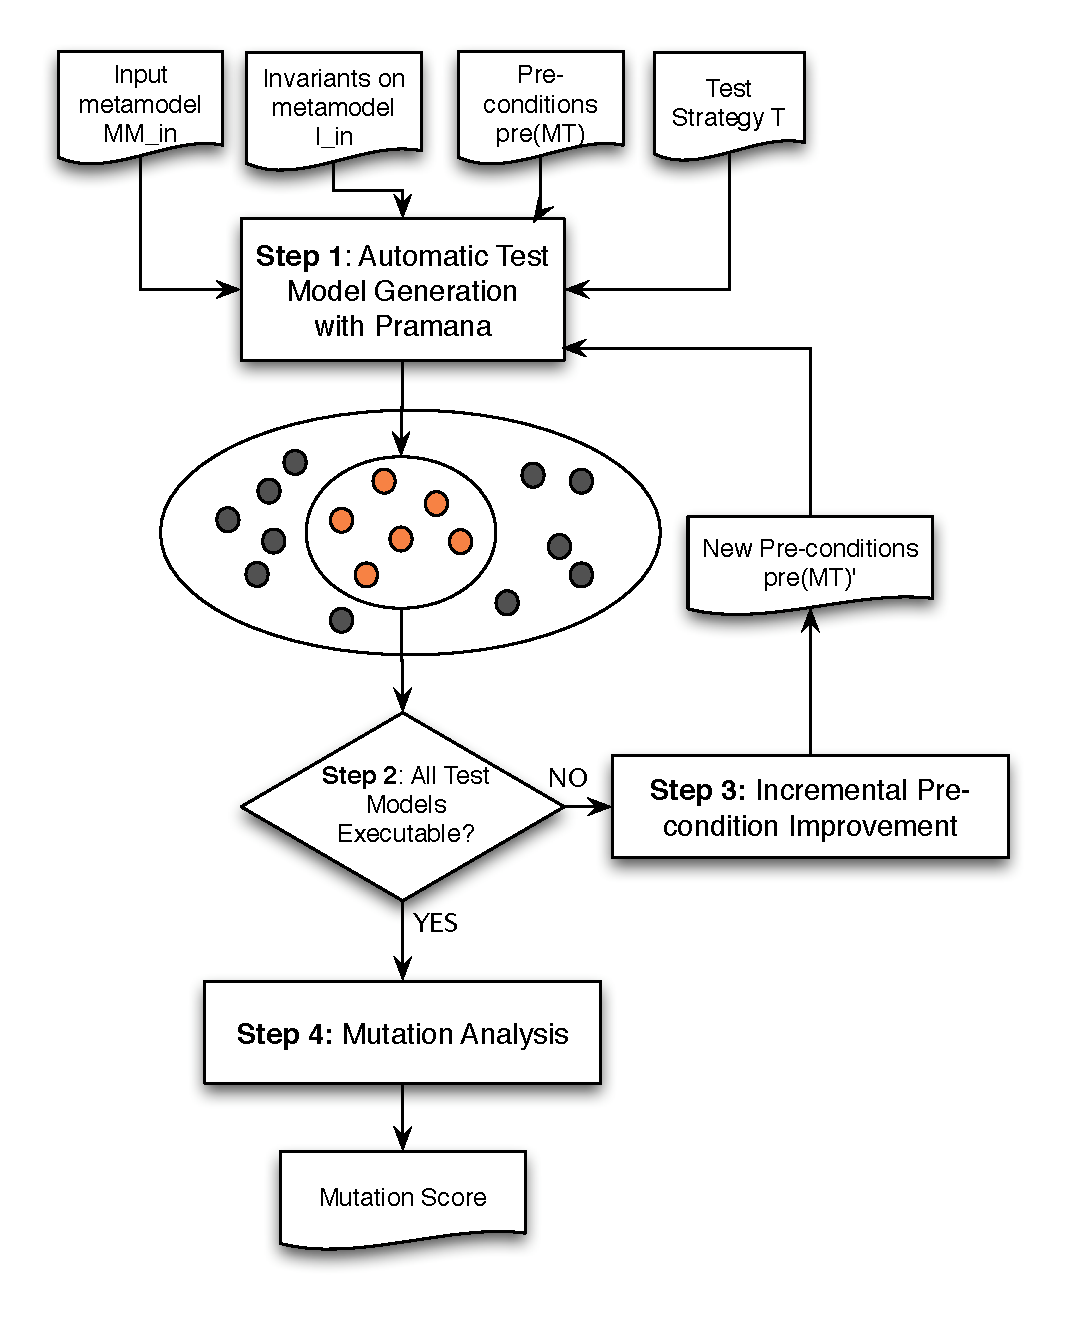
\includegraphics[height=5 in]{./figures/methodology.eps}
\end{center}
\caption{Methodology for Automatic Test Generation and Mutation Analysis}
\label{fig:methodology}
\end{figure*}

We outline the methodology for test generation  using {\Pramana} and empirical evaluation of the generated test models via mutation analysis in Figure \ref{fig:methodology}. The methodology uses  the foundational ideas we present in Section \ref{sec:Foundation} into a workflow. 

 Concisely, the test model generation workflow follows the steps:

\noindent \textbf{Step 1:} {\Pramana} transforms input metamodel $MM_{in}$, its invariants $I_{in}$, the transformation pre-condition $pre(MT)$ of transformation $MT$ and test strategy $T$ to an {\Alloy} model (details in Sections \ref{sec:sec:transfo2Alloy}, \ref{sec:sec:testStrategy}). {\Pramana} solves the {\Alloy} model to generate instances that are in the input domain of $MT$.

\noindent \textbf{Step 2:} 	We try to execute all test models generated by {\Pramana} as input to $MT$.

\noindent \textbf{Step 3:}   If all test models are not executable  in Step 2, then we incrementally create new pre-conditions for $MT$ called $pre(MT)'$. These pre-conditions are created from rejected test models. We describe incremental pre-condition improvement in Section \ref{sec:sec:precond}. We go to Step 1. Step 1 is executed using the a new source of constraints coming from $pre(MT)'$. 

\noindent \textbf{Step 4:} 	 If all test models are executable  in Step 2, we perform mutation analysis using the generated test models with respect to the model transformation $MT$. Mutation analysis is described in Section \ref{sec:sec:ma}.

\subsection{Incremental Pre-condition Improvement}
\label{sec:sec:precond}

The execution of a transformation helps us discover new pre-condition constraints $pre(MT)'$ for the transformation $MT$. In this sub-section we present the approach to systematically create new pre-conditions.

\begin{figure*} 
\begin{center}
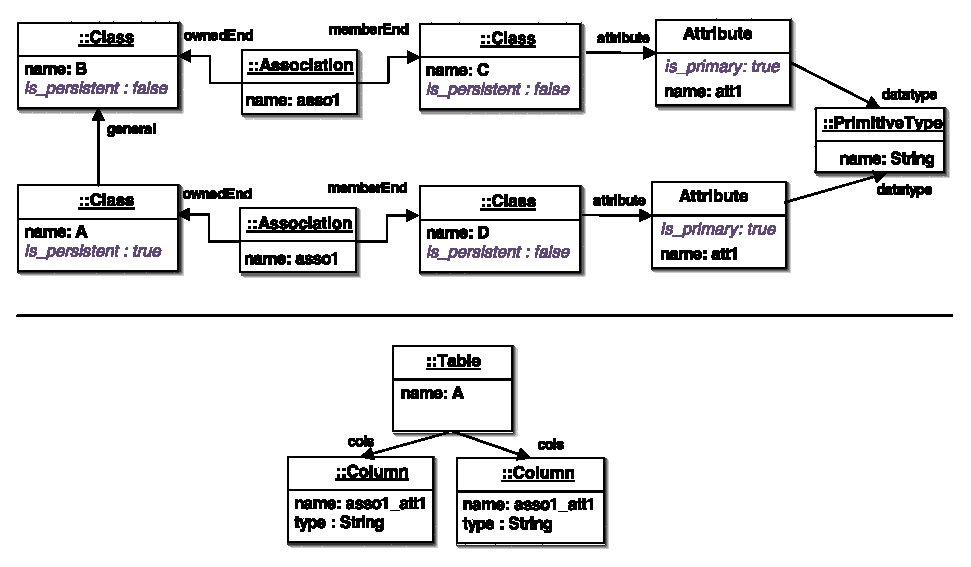
\includegraphics[width=6 in]{./figures/model-excerpt-for-constraint-improvment.eps}
\end{center}
\caption{Model Excerpt for Pre-condition Improvement}
\label{fig:modelExcerpt}
\end{figure*}

\noindent \textbf{Step 1:}  We execute the model transformation $MT$ with a test model $t$. 
\noindent \textbf{Step 2:}  The test model $t$ is rejected by the model transformation and the transformation terminates. The rejection of  a test model is often indicated by the raising of an exception by the transformation language. Some of the key sources for such rejections are:
					\begin{enumerate}
							\item \textbf{Insufficient memory} while creating modelling elements.
							\item \textbf{Infinite Loop} while navigating a test model.  For instance, this situation occurs when input models are navigated through a series of associations that can create loop structure in the transformation {\transfo}. These loops structures can navigation through diverse concepts such as  inheritance trees, associations, and type of attributes. The {\Kermeta} interpreter throws an  \textsf{StackOverflowError} exception when it detects such a problem. 
							\item \textbf{Transformation of an input model to an output model not in output domain}.  For instance, output models that do not satisfy the output meta-model specification and the post-condition $post(MT)$. In our case study, the transformation {\transfo} can produce ill-formed {\RDBMS} models. A typical example is when a table contains several columns with same name. We detect these inconsistencies by checking if output models conform to the output meta-model ({\ecore} model of the meta-model with invariants) and satisfy post-conditions of the model transformation. The Figure \ref{fig:modelExcerpt} illustrates this detection. It represents an excerpt (bottom part) of an output model produced by the original transformation of a generated (excerpt on the top part). 
					\end{enumerate}
					
\noindent \textbf{Step 3:}  We isolate inconsistent output models and corresponding test models. We then use a traceability mechanism and tool such as in \cite{glitia2008} to restrain the analysis of these models on excerpts such as the one illustrated in Figure \ref{fig:modelExcerpt}. Class named $A$ is transformed into one table because it is persistent. It redefined an association of the Class $B$. Two associations with the same name \emph{asso1} point  to classes with the same attribute/property \emph{att1}. Respecting the specification, the original transformations produces a table with two columns named \emph{asso1\_att1}. This does not conform to the {\RDBMS} meta-model and it is detected by our tool. Construction of such models can be prevented by generating objects with different names. 

\noindent \textbf{Step 4:}  We solve this inconsistency by creating a new pre-condition constraint that protects the transformation from executing such models. We also regenerate new models that satisfy the new pre-condition constraints. For instance, the faulty model excerpt in Figure \ref{fig:modelExcerpt} can help us produce a new pre-condition that states:

\emph{In the classes of an inheritance tree, two associations with the same name can't point to classes that have (or their parent) attributes with same names}.

Several new pre-conditions were discovered for the {\transfo} case study. We enlist nine newly discovered {\Alloy} facts in Appendix \ref{appendix:discoveredPrecondition} apart from the initial set of pre-condition constraints as shown in Appendix \ref{appendix:initialPrecondition}. These {\Alloy} facts can be easily expressed in {\OCL} to improve the pre-condition specification of {\transfo}. The conditions may even be applicable to commercial implementations of {\transfo}.


\section{Experiments}
\label{sec:Experiments}



\subsection{Experimental Setup and Execution}
\label{sec:sec:experiments}

We use the methodology in Section \ref{sec:Methodology} to compare coverage based test generation with unguided/random test model generation. 

Coverage based test strategies as previously introduced in Section \ref{sec:sec:testStrategy} consist of two test criteria {\AllRanges} and {\AllPartitions}.  These test criteria generate model fragments from an effective input meta-model. A test set satisfying {\AllRanges} must contain test models that contain all consistent model fragments from the {\AllRanges} criteria. Similarly, a test set satisfying {\AllPartitions} must contain all consistent model fragments generated from the {\AllPartitions} criteria.

We generate sets of test models based on factorial experimental design \cite{shari2005}. We consider the \emph{exact number of objects for each class} in the effective input meta-model as factors for experimental design. A factor level is the exact number of objects of a given class in a test model. These factors help study the effect of number of different types of objects on the mutation score. For instance, we can ask questions such as whether a large number of {\Association} objects have a correlation with the mutation score? The large of number {\Association} objects also indicates a highly connected {\UML} class diagram test model. We decide these factor levels by simple experimentation such as verifying if models can be generated in reasonable amount of time given that we need to generate thousands of test models in a few hours. We also want to cover a combination of a large number of varying factor levels. We have 8 different factor levels for the different classes in the {\UML} class diagram effective input meta-model as shown in Table \ref{table:mfFactorsa}. Other factors that may affect but are not considered for test model generation are the use different SAT solvers such as SAT4J, MiniSAT, or ZChaff, maximum time to solve, t-wise interaction between model fragments.

The {\AllRanges} criteria on the {\UMLCD} meta-model gives 15 consistent model fragments (see Table \ref{table:modelFrags}). We have 150 models in a set, where 10 non-isomorphic models satisfies each different model fragment. We generate 10 non-isomorphic models to verify that mutation scores do not drastically change within each solution. We synthesize 8 sets of 150 models using different levels for factors as shown in Table \ref{table:mfFactorsa} (see rows 1,2,3,4,5,6). The total number of models in these 8 sets is 1200. 

The {\AllPartitions} criteria gives 5 consistent model fragments. We have 50 test models in a set, where 10 non-isomorphic test models satisfies a different model fragment. We synthesize 8 sets of 50 models using factor levels shown in Table \ref{table:mfFactorsa}. The levels for factors for {\AllRanges} and {\AllPartitions} are the same. Total number of models in the 8 sets is 400. The selection of these factors at the moment is not based on a problem-independent strategy. 

We compare test sets generated using {\AllRanges} and {\AllPartitions} with unguided test sets. For each test set of coverage based strategies we generate an equal number of random/unguided models as a reference to qualify the efficiency of different strategies. Precisely, we have 8 sets of 150 unguided test models to compare with {\AllRanges} and 8 sets of 50 unguided test models to compare with {\AllPartitions}. We use the factor levels in Table \ref{table:mfFactorsa}.

\begin{table}

\caption{Factors and their Levels for  Test Sets}
\label{table:mfFactorsa}
\begin{tabular}[a]{p {2 cm}  l  l  l  l  l l  l  l  l}
%& & &\textbf{(a)} & & & & & &
\hline
%				&   &   &   &    & \textbf{Sets}   &    &   &    \\ 
\textbf{Factors} &&  S1 & S2  &  S3 &  S4  &  S5  &  S6  &  S7 &  S8  \\ \hline 
\textbf{\#ClassModel} && 1 & 1 & 1 & 1 & 1 & 1 & 1 & 1 \\ 
\textbf{\#Class}  &&  5 & 5  & 15 & 15 & 5 & 15 & 5 & 15 \\ 
\textbf{\#Association} && 5 & 15 & 5 & 15  & 5  & 5  & 15  & 15 \\  
\textbf{\#Attribute}  && 25 & 25 & 25 & 25 & 30  & 30 & 30 & 30 \\ 
\textbf{\#PrimitiveDataType} && 4 & 4 & 4 & 4 & 4 & 4 & 4 & 4 \\ 
\textbf{Bit-width Integer}  && 5 & 5 & 5 & 5 & 5 & 5 & 5 & 5\\ 
\textbf{\#Models/Set} {\AllRanges} && 15 & 15 & 15 & 15 & 15 & 15 & 15 & 15 \\ 
\textbf{\#Models/Set} {\Unguided} && 15 & 15 & 15 & 15 & 15 & 15 & 15 & 15 \\ 
\textbf{\#Models/Set} {\AllPartitions}  && 5 & 5 & 5 & 5 & 5 & 5 & 5 \\ 
\textbf{\#Models/Set} {\Unguided}  && 5 & 5 & 5 & 5 & 5 & 5 & 5 \\ \hline
\end{tabular}

\end{table}

\begin{table*} 
	%\vspace{-1 cm}
%% increase table row spacing, adjust to taste
\renewcommand{\arraystretch}{1}
\renewcommand{\arrayrulewidth}{1 pt}
\caption{Mutation Scores in Percentage for All Test Model Sets}
\label{table:mutationScores}
\centering
\begin{tabular}{ l  l l l l l l l l }
\hline
\textbf{Set} & 1 & 2 & 3 & 4 & 5 & 6 & 7 & 8\\ \hline
 \textsf{Unguided} \textbf{150 models/set in 8 sets} & 68.56 & 69.9 & 68.04 & 70.1 & 70.1 & 68.55 & 69 & 70.1 \\
 {\AllRanges} \textbf{150 models/set in 8 sets}  &  88.14 & 92.26  &  81.44 & 85 & 91.23 & 80.4 & 91.23 &  88.14 \\ 
 \textsf{Unguided} \textbf{50 models/set in 8 sets} & 70.1 & 62.17 & 68.04 & 70.1 & 65.46 & 68.04 & 69.94 & 70.1 \\ 
{\AllPartitions} \textbf{50 models/set in 8 sets} & 90.72 & 93.3 & 84.53 & 87.62  & 87.62  & 82.98 & 92.78& 88.66 \\ \hline
\end{tabular}

\end{table*}

To summarize, we generate a total of 3200  models using an Intel(R) Core$^{TM}$ 2 Duo processor with  4GB of RAM. We perform mutation analysis of these sets to obtain mutation scores on a grid of 10 Intel Celeron 440 high-end computers. The computation time for generating 3200 models was about 3 hours and mutation analysis took  about 1 week. We discuss the results of mutation analysis in the following section. 

\subsection{Results and Discussion}
\label{sec:results}


Mutation scores for {\AllRanges} test sets are shown in Table \ref{table:mutationScores} (row 2). Mutation scores for test sets obtained using {\AllPartitions} are shown in Table \ref{table:mutationScores} (row 4). We discuss the effects of the influencing factors on the mutation score:
\begin{itemize}
	\item The number of {\Class} objects and {\Association} objects has a strong correlation with the mutation score. There is an increase in mutation score with the level of these factors. This is true for sets from unguided and model fragments based strategies. For instance, the lowest mutation score using {\AllRanges} is 80.41 \%. This corresponds to set 1 where the factor levels are 1,5,5,25,4,5  (see Column for set 1 in Table \ref{table:mfFactorsa}) and highest mutation scores are 91,24 and 92,27\% where the factor levels are 1,15,5,25,4,5 and 1,5,15,25,4,5 respectively  (see Columns for set 3 and set 7 in Table \ref{table:mfFactorsa}).

%	\item We observe a strong correlation of the mutation score with the number of {\Class} and {\Association} objects due to the nature of the injected mutation operators. The  creational, navigational, and filtering mutation operators injected in the model transformation are killed by input test models  using a large number of {\Class} and {\Association} objects. However, we see that unguided models with both large and small number of {\Class} and {\Association} objects are not able to have a mutation score above 70.1\%. There is a clear need for more knowledge to improve this mutation score. 
	\item We observe that {\AllPartitions} test sets containing only 50 models/set gives a score of maximum 93.3\%. The {\AllPartitions} strategy demonstrates that knowledge from two different partitions satisfied by one test model greatly improves bug detecting efficiency. This also opens a new research direction to explore: Finding strategies to combine model fragments to guide generation of  smaller sets of complex test models with better bug detecting effectiveness.
\end{itemize}

We compare unguided test sets with model fragment guided sets in the \emph{box-whisker} diagram shown in Figure \ref{fig:whisker}. The box whisker diagram is useful to visualize groups of numerical data such as mutation scores for test sets. Each box in the diagram is divided into lower quartile (25\%), median, upper quartile (75\% and above), and largest observation and contains statistically significant values. A box may also indicate which observations, if any, might be considered outliers or whiskers. In the box whisker diagram of Figure \ref{fig:whisker} we shown 4 boxes with whiskers for unguided sets and sets for {\AllRanges} and {\AllPartitions}. The X-axis of this plot represents the strategy used to select sets of test models and the Y-axis represents the mutation score for the sets.

\begin{figure*} 

\begin{center}
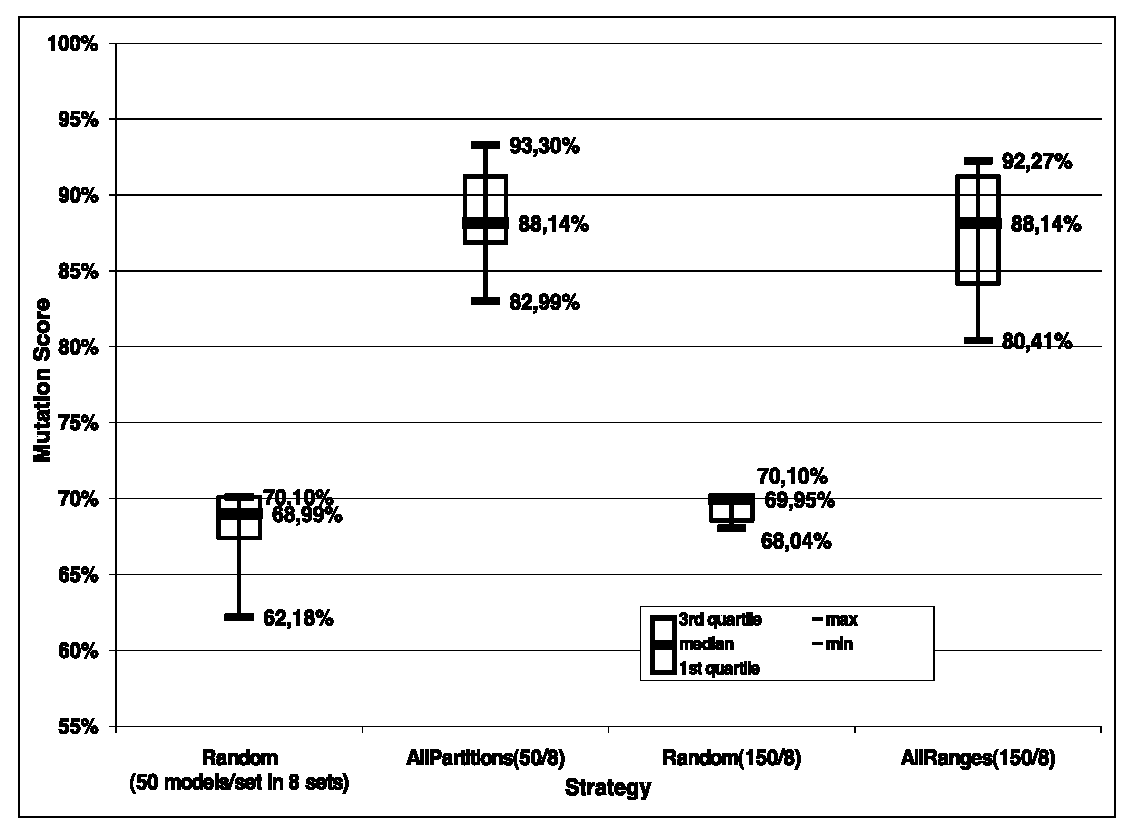
\includegraphics[width=5 in]{./figures/boxplot.eps}
\end{center}
\caption{Box-whisker Diagram to Compare Automatic Model Generation Strategies}
\label{fig:whisker}

\end{figure*}


We make the following observations from the box-whisker diagram:
\begin{itemize}
	\item Both the boxes of {\AllRanges} and {\AllPartitions} represent mutation scores higher than corresponding unguided sets.
	\item The high median mutation scores for strategies {\AllRanges} 88.14\% and {\AllPartitions} 88.14\% indicate that both these strategies return consistently good test sets.
	\item The small size of the box for {\AllPartitions} compared to the {\AllRanges} box indicates its relative convergence to good sets of test models.
	\item The small set of 50 models using {\AllPartitions} gives mutations scores equal or greater than 150 models/set using {\AllRanges}. This implies that it is a more efficient strategy for test model selection. The main consequence is a reduced effort to write corresponding \emph{test oracles} \cite{mottu2008} with 50 models compared to 150 models.
	\item Despite the generation of multiple solutions (10 solutions  for each model fragment or an empty fragment for unguided generation) for each strategy we see a consistent behaviour in the mutation scores. There is no large difference in the mutation scores especially for unguided generation. The median is 69\% and the mutation scores range between 68\% and 70\%. The {\AllRanges} and {\AllPartitions} vary a little more in their mutation scores due to a larger coverage of the effective input meta-model.
\end{itemize}	

The freely and automatically obtained knowledge from the input meta-model using the MMCC algorithm shows that  {\AllRanges} and {\AllPartitions} are successful strategies to guide test generation. They have higher mutation scores with the same sources of knowledge used to generate unguided test sets. A manual analysis of the test models reveals that injection of inheritance via the parent relation in model fragments results in higher mutation scores. Most unguided  models do not contain inheritance relationships as it is not imposed by the meta-model.
 
 What about the 7\% of the mutants that remain alive given that the highest mutation score is 93.3\%? We note by an analysis of the live mutants that they are the same for both {\AllRanges} and {\AllPartitions}. There remain 19 live mutants in a total of 200 injected
mutants (with 6 equivalent mutants). In the median case both AllRanges and AllPartitions strategy give a mutation score of 88.14\%. The live mutants in the median case are mutants not killed due to fewer objects in models.

To consistently achieve a higher mutation score we need more CPU speed, memory and parallelization to efficiently generate larger test models and perform mutation analysis on them. This extension of our work has not be been explored in the paper. It is important for us to remark that some live mutants can only be killed with more information about the model transformation such as those derived from its requirements specification. For instance, one of the remaining live mutant requires a test model with a class containing several primitive type attributes such that at least one is a primary attribute. A test model that satisfies such a requirement requires the combination of model fragments imposing the need for several attributes in a class A, attributes of class A must have  primitive types, at least one primary attribute in the class A, and at least one non-primary attribute in the class A. This requirement can either be specified by manually creating a combination of fragments or by developing a better general test strategy to combine multiple model fragments. In another situation, we observe that not all model fragments are consistent with the input domain and hence they do not really cover the entire meta-model. Therefore, we miss killing some mutants. This information could help improve partitioning and combination strategies to generate better test sets.


\section{Related Work}
\label{sec:RelatedWork}


We explore three main areas of related work : test criteria, automatic test generation, and qualification of strategies. 

The first area we explore is work on test criteria in the context of model transformations in {\MDE}. Random generation and input domain partitioning based test criteria are two widely studied and compared  strategies in software engineering (non {\MDE})  \cite{vagoun1996}  \cite{elaine1991} \cite{Gutjahr99partitiontesting}. To extend such test criteria to {\MDE} we have presented in \cite{franck2007} input domain partitioning of input meta-models in the form of model fragments. However, there exists no experimental or theoretical study to qualify the approach proposed in \cite{franck2007}.

Experimental qualification of the test strategies require techniques for automatic model generation. Model generation is more general and complex than generating integers, floats, strings, lists, or other standard data structures such as dealt with in the Korat tool of Chandra et al. \cite{chandra2002}. Korat is faster than {\Alloy} in generating data structures such as binary trees, lists, and heap arrays from the Java Collections Framework but it does not consider the general case of models which are arbitrarily constrained graphs of objects. The constraints on models makes model generation a different problem than generating test suites for context-free grammar-based software \cite{hen2005} which do not contain domain-specific constraints. 

  Test models are complex graphs that must conform to an input meta-model specification, a transformation pre-condition and additional knowledge such as model fragments to help detect bugs. In \cite{brottier2006} the authors present an automated generation technique for models that conform only to the class diagram of a meta-model specification. A similar methodology using graph transformation rules is presented in \cite{ehrig2006}. Generated models in both these approaches do not satisfy the constraints on the meta-model. In \cite{sen2007} we present a method to generate models given partial models by transforming the meta-model and partial model to a {\textCLP} ({\CLP}). We solve the resulting {\CLP} to give model(s) that conform to the input domain. However, the approach does not add new objects to the model. We assume that the number and types of models in the partial model is sufficient for obtaining complete models. The constraints in this system are limited to first-order horn clause logic.  In \cite{sen2008} we have introduce a tool {\Cartier} based on the constraint solving system {\Alloy} to resolve the issue of generating models such that constraints over both objects and properties are satisfied simultaneously. In this paper we use {\Cartier} to systematically generate several hundred models driven by knowledge/constraints of model fragments \cite{franck2007}. Statistically relevant test model sets are generated from a factorial experimental design \cite{shari2005} \cite{walter1955}.% \cite{hoskins2004}.

The qualification of a set of test models can be based on several criteria such as code and rule coverage for white box testing, satisfaction of post-condition or mutation analysis for black/grey box testing. In this paper we are interested in obtaining the relative adequacy of a test set using mutation analysis \cite{demillo1978}. In previous work \cite{mottu2006} we extend mutation analysis to {\MDE} by developing mutation operators for model transformation languages. We qualify our approach using a representative transformation {\UMLCD} models to {\RDBMS} models called {\transfo} implemented in the transformation language Kermeta \cite{muller2005}. This transformation \cite{bezivin2005} was proposed in the MTIP Workshop in MoDeLs 2005 as a comprehensive and representative case study to evaluate model transformation languages.

\section{Conclusion}
\label{sec:Conclusion}

Testing model transformations  presents the challenging problem of developing approaches to automatically generate effective test models. In this paper we present {\Pramana}, a tool to generate models conforming in the input domain of a transformation and guided by different coverage criteria.  First, {\Pramana} helps us precisely specify the input domain of a model transformation incremental pre-condition improvement.  Second, we use {\Pramana} to generate sets of test models that compare coverage and unguided strategies for model generation. All test sets using these strategies detect faults given by their mutation scores.  The comparison of coverage strategies with unguided generation taught us that both strategies {\AllPartitions} and {\AllRanges} look very promising. Coverage strategies give a maximum mutation score of 93\% compared to a maximum mutation score of 70\% in the case of unguided test sets. We observe that mutation scores do not vary drastically despite the generation of multiple solutions for the same test strategy.  We conclude from our experiments that the {\AllPartitions} strategy is a promising strategy to consistently generate a small test of test models with a good mutation score. However, to improve effectiveness of test sets we might require effort from the test designer to obtain test model knowledge/test strategy that take the internal model transformation design requirements into account. The experiments in this paper were performed based on the mutation analysis of {\transfo} written in the language {\Kermeta}. In future, we intend to develop mutation analysis tools for various mature model transformation languages. The automatic mutation analysis tool will help us perform experiments using a number of transformation case studies. Applying our approach to large input metamodels such as the {\UML} is a challenge in scaling our approach. We intend to leverage our recently developed technique called \emph{metamodel pruning} \cite{sen2009b} to extract a small subset of large metamodel such as {\UML} which is conducive to constraint solving in {\Pramana} and consequently model generation for large input metamodels. 


%
% BibTeX users please use
% \bibliographystyle{}
% \bibliography{}
\appendix


\section{{\Alloy} Model Synthesized by {\Cartier}}
\label{appendix:mainmodel}

\lstinputlisting[language=Alloy, basicstyle=\tiny,
style=nonumbers, frame=single, framerule=0.2pt, captionpos=b,
caption={{\Alloy} Model for {\UML} Class Diagram}, label={listing:alloyModel}]{./listings/alloyModel.tex}


\section{Initial Set of Pre-conditions}
\label{appendix:initialPrecondition}

\lstinputlisting[language=Alloy, basicstyle=\tiny,
style=nonumbers, frame=single, framerule=0.2pt, captionpos=b,
caption={Initial pre-conditions as {\Alloy} facts }, label={listing:precond}]{./listings/initialPreconditions.tex}

\section{Discovered Set of Pre-conditions}
\label{appendix:discoveredPrecondition}

\lstinputlisting[language=Alloy, basicstyle=\tiny,
style=nonumbers, frame=single, framerule=0.2pt, captionpos=b,
caption={Discovered pre-conditions as {\Alloy} facts }, label={listing:discprecond}]{./listings/discoveredPreconditions.tex}


\bibliographystyle{splncs}
\bibliography{Prop-SoSym}


\end{document}

% end of file template.tex

